% Chapter 11 of Volume III (key pf): The Polya frequency ladder: certified log concavity, the detection rung and the heat flow. Sources: misc/reviews/nick-volume3/vol3/ch4_path.tex (lines per STRUCTURE.md Chapter 11), reports U04 (M1 to M11) and V3B (P01 to P38), verification W1 (V1, V4), certificate PF2 (CERTIFICATE.md) audited by PF2_audit.md. 17 Nov 2026.
\label{p:ch:path}
% Audited: PF2_audit.md (Opus), astra/V3P/report.md (GPT), both pass
% Figures dropped: the draft's fig_cert (plots the draft's own certified bounds, which differ from those of the rebuilt certificate) and fig_heat (its right panel plots the first pair heights 32.9 and 49.8 of the draft table, the correct values are 33.1 and 49.7); both must be redrawn if wanted.
% Normalisation: xi is the book's xi, with Riemann's factor 1/2, so xi(1/2)=0.4971...; omega(t)=xi(1/2)/xi(1/2+t), the residues c_n and all minors are unchanged by the factor. The book's phi(t^2) of pol:prop:pf is omega(t) here; the draft's F is the book's f_X. Heat time as in ch21 (H_0(z)=Xi(z/2)/8, zeros z=2 gamma), the draft's flow equations already agree with it.

This chapter takes one formulation of RH, total positivity, and asks what can be proved and computed about it. Its object is a single explicit function on the real line,
\[
F(x)=\frac1\pi\int_0^\infty\cos(tx)\,\omega(t)\,\mathrm dt,\qquad \omega(t)=\frac{\xi(\frac12)}{\xi(\frac12+t)},
\]
which is the density $f_X$ of Proposition~\ref{pol:prop:pf}. It is built from $\xi$ on the real axis alone. RH is the statement that $F$ is a P\'olya frequency function. The condition is a ladder of rungs, each a family of determinant inequalities for $F$.

Nothing here proves RH. The approach of Sections~\ref{p:sec:far}, \ref{p:sec:detect} and \ref{p:sec:heat} to \ref{p:sec:sharp} is from an unrefereed note of Polson (November 2026). The certificate of Section~\ref{p:sec:m1} follows that note's strategy, but its quadrature lemma, ellipse constants, zero completeness and tail bounds were rebuilt and rerun, and the certificate as printed is ours.

\paragraph{Status of the main statements} The table sorts them by level of evidence. Floating point values are marked computed, and ball arithmetic is marked certified.
\begin{center}
\footnotesize
\begin{tabular}{p{0.34\textwidth}p{0.56\textwidth}}
\toprule
level & statements\\
\midrule
proved & far field of each fixed configuration, for $k$ up to about $10^{13}$ (Theorem~\ref{p:thm:farpfk}); detection rung (Theorem~\ref{p:thm:detect}); the PF reading of the heat flow (Theorem~\ref{p:thm:heat}); the critical point test (Proposition~\ref{p:prop:crit})\\
certified & $F>0$ and $(\log F)''<0$ on $\mathbb R$ (Theorem~\ref{p:thm:m1})\\
computed & the Davenport Heilbronn control at rung $44$; first pairs off the line for $-4\le t\le-0.1$; minors of $F_{-4}$ and $F_{-2}$; the zero flow for $-4\le t<0$\\
computed, truncated & the Csordas Smith Varga quantities of Table~\ref{p:tab:lehmer} (not bounds: the tail of the zeros is not bounded here)\\
open & PF$_k$ for $k\ge3$ on $\mathbb R$; sharpness of the rung bound; the growth of the failing rung\\
\bottomrule
\end{tabular}
\end{center}

\section{The ladder}\label{p:sec:target}

A function $F\colon\mathbb R\to\mathbb R$ is PF$_k$ if every minor of order at most $k$ is nonnegative: for every $j\le k$ and all $x_1<\dots<x_j$, $y_1<\dots<y_j$,
\[
\det\big[F(x_i-y_l)\big]_{i,l=1}^j\ \ge\ 0 .
\]
The condition on orders below $k$ is part of the definition. With only the order $k$ the ladder would not be nested, because $-F$ has positive determinants of every even order when $F$ is a strictly totally positive density. PF$_1$ is $F\ge0$. For a positive $F$, PF$_2$ is log concavity. $F$ is a P\'olya frequency function (PF$_\infty$) if it is PF$_k$ for every $k$. By Proposition~\ref{pol:prop:pf}, RH holds if and only if $F$ is PF$_\infty$, and then $F$ is the density of $\sum_{\gamma>0}L_\gamma/\gamma$ with independent standard Laplace variables $L_\gamma$.

Write $\Xi(z)=\xi(\frac12+iz)$, an even entire function of order one, real on the real axis, whose zeros $\pm\gamma$ correspond to the zeros $\rho=\frac12+i\gamma$ of $\zeta$. We write $\gamma_1<\gamma_2<\dots$ for the positive real zeros of $\Xi$ (these are the ordinates of the zeros on the line).

\begin{lemma}\label{p:lem:phipath}
For real $t$, $0<\omega(t)\le1$, $\omega(0)=1$, $\omega$ is even and decreasing on $[0,\infty)$, and for $t>\frac12$, with $\sigma=\frac12+t$,
\[
\omega(t)\le g(t)=\frac{2\,\xi(\frac12)\,\pi^{\sigma/2}}{\sigma(\sigma-1)\,\Gamma(\sigma/2)} .
\]
Consequently $F$ is an even entire function with $\int_{\mathbb R}F=1$, $F''(0)<0$ and $|F^{(m)}(x)|\le M_m=\frac1\pi\int_0^\infty t^m\omega(t)\,\mathrm dt$ for real $x$.
\end{lemma}

\begin{proof}
$\omega(t)=\mathbb Ee^{-t^2Y}$ in the notation of Proposition~\ref{pol:prop:pf}, which gives positivity, evenness, monotonicity and the bound by $1$. For $\sigma>1$, $\zeta(\sigma)\ge1$ gives $\xi(\sigma)\ge\frac12\sigma(\sigma-1)\pi^{-\sigma/2}\Gamma(\sigma/2)$, hence the bound by $g$. The function $g$ decays like a gamma factor, so $F$ is entire, the derivatives may be taken under the integral, and $F(x)=\frac1{2\pi}\int_{\mathbb R}e^{itx}\omega(t)\,\mathrm dt$ has $\int F=\omega(0)=1$. The bound for $F^{(m)}$ is the trivial bound on the integral, and $F''(0)<0$ is Lemma~\ref{pol:lem:origin}.
\end{proof}

\section{The far field}\label{p:sec:far}

\subsection{The residue expansion}

We use Lemma~\ref{pol:lem:residue} in the following form. Let $T>0$ be such that the zeros of $\xi$ with $|\Im s|<T$ are exactly $\frac12\pm i\gamma_n$, $n\le N$, all simple, and let $T$ not be an ordinate. Then for $x>0$ and $k\ge0$,
\begin{equation}\label{p:eq:residue}
F^{(k)}(x)=\sum_{n=1}^Nc_n(-\gamma_n)^ke^{-\gamma_nx}+R_k(x),\qquad c_n=-\frac{\xi(\frac12)}{\Xi'(\gamma_n)},\qquad |R_k(x)|\le K_ke^{-Tx},
\end{equation}
with $K_k=\frac1\pi\int_0^\infty|u-iT|^k\,|\omega(u-iT)|\,\mathrm du$. The proof moves the line of integration of $\frac1{2\pi}\int e^{-itx}\omega(t)\,\mathrm dt$ to $\Im t=-T$, crossing the simple poles $t=-i\gamma_n$. Zeros are verified simple and on the line up to height $3\times10^{12}$ \cite{PT21}, so \eqref{p:eq:residue} holds unconditionally for every such $T$ that is not an ordinate. With the first $1703$ zeros it reproduces the Fourier computation of $F$: at $x=1$ both give $2.45157853995\times10^{-4}$ (computed, $12$ digits).

\begin{figure}[t]
\centering
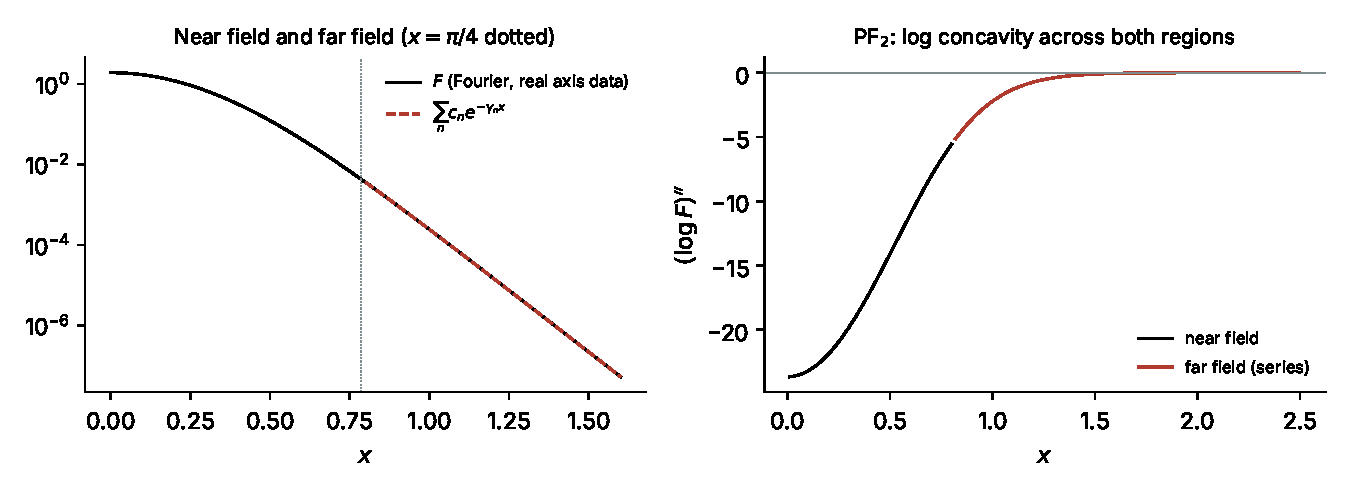
\includegraphics[width=\textwidth]{fig/v3/pf_fig_far.pdf}
\caption{Left: $F$ from real axis data, and the residue series, used for $x>\pi/4$ (dotted). Right: $(\log F)''$ in the near field (Fourier) and in the far field (series).}
\label{p:fig:far}
\end{figure}

\subsection{The radius \texorpdfstring{$\pi/4$}{pi/4}}

The residue $|c_n|=\xi(\frac12)/|\Xi'(\gamma_n)|$ is of size $e^{\pi\gamma_n/4}$ up to powers of $\gamma_n$ on average, since $\Xi(z)$ decays like $z^{7/4}e^{-\pi z/4}$ on average.
The infinite series is therefore useful only for $x>\pi/4$. That it converges there is heuristic: it needs $|\zeta'(\rho)|\ge e^{-o(\gamma)}$ and simplicity of every zero, neither of which is known even under RH. It diverges for $x<\pi/4$ unconditionally, from the polynomial upper bound for $\zeta'$ on the line. Inside that radius $F$ is not a sum over zeros. All the arguments below use the finite expansion \eqref{p:eq:residue} with its remainder.

\subsection{The sign rule}

\begin{proposition}\label{p:prop:signrule}
Let $\gamma_1<\dots<\gamma_K$ be the first $K$ positive zeros of $\Xi$, and suppose they are real and simple, so that $\Xi$ has no zero in $(0,\gamma_1)$. Then $c_1,\dots,c_K$ alternate in sign, and $c_1>0$.
\end{proposition}

\begin{proof}
$c_n=-\xi(\frac12)/\Xi'(\gamma_n)$ and $\Xi$ is real on the real axis. Between consecutive simple real zeros $\Xi$ keeps one sign, so $\Xi'$ alternates. Since $\Xi(0)=\xi(\frac12)>0$ and $\Xi$ is positive on $[0,\gamma_1)$, $\Xi'(\gamma_1)<0$ and $c_1>0$.
\end{proof}

We verified the alternation for $n\le1703$ (computed), and the certified values for $n\le13$ are in Table~\ref{p:tab:res}. The real residues alternate whether or not a complex quadruple sits between the real zeros, since $\Xi$ changes sign only at real zeros of odd order. An off line pair adds two nonreal residues and leaves the alternation of the real ones intact. So the sign pattern of the real residues does not detect an off line zero.

\subsection{Every rung, for each fixed configuration}

The two term case is Lemma~\ref{pol:lem:two}. With $S_k=\sum c_n(-\gamma_n)^ke^{-\gamma_nx}$, symmetrisation gives $S_0S_2-S_1^2=\frac12\sum_{n,m}c_nc_m(\gamma_n-\gamma_m)^2e^{-(\gamma_n+\gamma_m)x}$, and for $T\in(\gamma_2,\gamma_3)$
\[
(\log F)''(x)=\frac{c_2}{c_1}(\gamma_2-\gamma_1)^2e^{-(\gamma_2-\gamma_1)x}\big(1+O(e^{-\delta x})\big),\qquad \delta>0 .
\]
Since $c_2/c_1<0$, $F$ is log concave for large $x$, unconditionally. The general case is the following theorem, which completes the sketch after Theorem~\ref{pol:thm:pf2}.

\begin{theorem}\label{p:thm:farpfk}
Let $k\ge1$ and let $T>\gamma_k$ be such that the zeros of $\xi$ with $|\Im s|<T$ are exactly $\frac12\pm i\gamma_n$, $n\le k$, simple, with $T$ not an ordinate. Fix $x_1<\dots<x_k$ and $y_1<\dots<y_k$. Then $\det[F(x_i+L-y_l)]>0$ for all sufficiently large $L$.
\end{theorem}

\begin{proof}
By \eqref{p:eq:residue}, $F(x+L)=\sum_{n\le k}c_ne^{-\gamma_n(x+L)}+O(e^{-T(x+L)})$ uniformly for $x$ in a bounded set. The main part is a product kernel, and the Cauchy Binet formula gives
\begin{multline*}
\det\Big[\sum_{n\le k}c_ne^{-\gamma_n(x_i+L)}e^{\gamma_ny_l}\Big]\\=e^{-(\gamma_1+\dots+\gamma_k)L}\prod_{n\le k}c_n\,\det[e^{-\gamma_nx_i}]\,\det[e^{\gamma_ny_l}].
\end{multline*}
$\det[e^{\gamma_ny_l}]>0$ because the exponential kernel is totally positive. $\det[e^{-\gamma_nx_i}]$ has sign $(-1)^{k(k-1)/2}$ (reverse the order of the rows). By Proposition~\ref{p:prop:signrule}, $\prod c_n$ has the same sign $(-1)^{k(k-1)/2}$, so the main term is positive and of size $e^{-(\gamma_1+\dots+\gamma_k)L}$. Expand the full determinant by multilinearity in the columns. A term with $r\ge1$ remainder columns is bounded by $e^{-rTL}$ times the largest main contribution of $k-r$ columns, which is $O(e^{-(\gamma_1+\dots+\gamma_{k-r})L})$. Every such term is $O(e^{-(\gamma_1+\dots+\gamma_{k-1}+T)L})$, which is smaller since $T>\gamma_k$.
\end{proof}

Two limits of this result matter. The theorem decides each fixed configuration only for $L$ large enough, not uniformly in the configuration, and it says nothing about configurations in which some differences $x_i-y_l$ are small and others large. For each fixed configuration the far field of rung $k$ is therefore decided by the first $k$ zeros, which are verified for $k$ up to about $10^{13}$.

\section{The near field}\label{p:sec:near}

For $|x|<\pi/4$ the residue series diverges and all zeros act at once. With $F$ computed from real axis data (computed):
\begin{itemize}
\item $(\log F)''\le-5.57$ on $[0.01,0.8]$ % UNVERIFIED: only the value at 0.8 was verified (W1)
, and Theorem~\ref{p:thm:m1} below makes log concavity rigorous on $\mathbb R$.
\item We sampled $2\times10^5$ random ordered configurations in $[-0.6,0.6]$ for each of $k=2,3,4$. No $k\times k$ minor was negative beyond $7\times10^{-6}$ of its scale, which is the size of the interpolation error. % UNVERIFIED: not rerun in W1
\end{itemize}
This is evidence, not proof.

\paragraph{Stress points} After removing the trend in $\log|c_n|$, the largest excess residues come from close pairs of zeros (Figure~\ref{p:fig:stress}): $1329.04$ and $1329.21$, and $1977.17$ and $1977.27$. A close pair makes $\Xi'$ small at both zeros, so it inflates two consecutive residues of opposite sign. These are Lehmer type pairs. Such pairs gave the classical lower bounds on the de Bruijn Newman constant (Table~\ref{tab:ch21:hist}).

\begin{figure}[t]
\centering
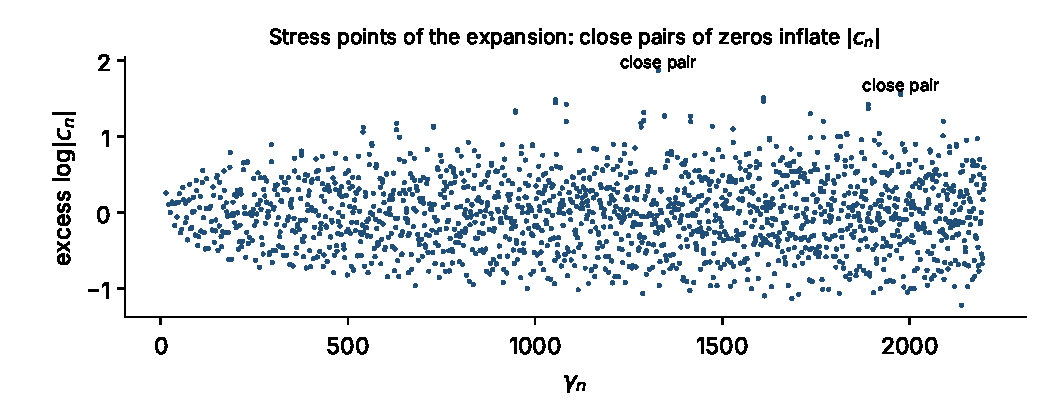
\includegraphics[width=\textwidth]{fig/v3/pf_fig_stress.pdf}
\caption{Excess of $\log|c_n|$ over its trend for the first $1703$ zeros. The spikes are close pairs of zeros.}
\label{p:fig:stress}
\end{figure}

\section{The P\'olya density is strictly log concave (certified)}\label{p:sec:m1}

\begin{theorem}[certified]\label{p:thm:m1}
The Riemann density $F=f_X$ is strictly log concave on $\mathbb R$: $F>0$ and $(\log F)''<0$ at every real point. In particular $F$ is PF$_1$ and PF$_2$, and, by Ibragimov's theorem \cite{Ibragimov56}, the law with characteristic function $\omega$ is strongly unimodal.
\end{theorem}

This answers Problem~\ref{pol:op:pf2}, for PF$_2$. Theorem~\ref{pol:thm:pf2} gave a floating point certificate, and the proof here uses interval enclosures at every step. Certified here means ball arithmetic only, resting on the trusted base listed at the end of the section.

\paragraph{Strategy} Put $G=FF''-F'^2$, so that log concavity is $G<0$. $F$ is even, so it is enough to treat $x\ge0$. We split at $X_1=2$.
\begin{itemize}
\item Near field, $0\le x\le2$. Taylor models of $F,F',F''$ on $400$ cells of width $\frac1{200}$, built from derivatives $F^{(j)}(a)$, $j\le19$, obtained by quadrature with a proved error bound on Bernstein ellipses.
\item Far field, $x\ge2$. The residue expansion \eqref{p:eq:residue} with the thirteen zeros of height below $60.09$, and a proved remainder.
\end{itemize}
The zeros enter in two places: completeness of the list of thirteen, which is proved below by the argument principle, and the absence of zeros of $\xi(\frac12+t)$ in the ellipses of the near field. Floating point values appear only in displays, in one integrator tolerance and in diagnostic checks; no sign or bound is decided by them.

\subsection{Zero data}

Let $T=60.09$. The zeros $\gamma_1,\dots,\gamma_{14}$ are first located by Arb's zero finder, used only as a starting guess. For $n\le14$ the interval $I_n=[\gamma_n-10^{-20},\gamma_n+10^{-20}]$ is certified to contain exactly one zero, which is simple: $\Xi$ has strictly opposite signs at its endpoints and $\Xi'$ has one strict sign on $I_n$. The intervals are disjoint and increasing, and $T$ lies between $I_{13}$ and $I_{14}$. The residues $c_n$ are enclosed, and they alternate in sign with $c_1>0$.

Completeness is proved, not cited. Let $\mathcal R$ be the rectangle $-1<\Re s<2$, $|\Im s|<T$. Integrating $\xi'/\xi$ around the boundary in ball arithmetic gives $26.000000\pm4.3\times10^{-7}$ zeros in $\mathcal R$. The $26$ zeros $\pm\gamma_1,\dots,\pm\gamma_{13}$ are distinct, so they are all the zeros in $\mathcal R$, all simple and on the line, and no zero has $|\Im s|<\gamma_1=14.13$. Outside $\mathcal R$ there are none of height below $T$: for $\Re s\ge2$, $|\zeta(s)|\ge2-\zeta(\sigma)>0$ and the other factors of $\xi$ do not vanish, and for $\Re s\le-1$ use $\xi(s)=\xi(1-s)$. This uses only heights below $60.09$, and uses that $\xi$ is real on the real axis, not RH.

\begin{table}[t]
\centering
\footnotesize
\begin{tabular}{rcc}
\toprule
$n$ & $\gamma_n$ & $c_n$\\
\midrule
1 & 14.13472514 & $3.59524\times10^{2}$\\
2 & 21.02203964 & $-2.80072\times10^{4}$\\
3 & 25.01085758 & $3.92918\times10^{5}$\\
4 & 30.42487613 & $-2.06128\times10^{7}$\\
$\vdots$ & $\vdots$ & $\vdots$\\
13 & 59.34704400 & $4.39841\times10^{16}$\\
\bottomrule
\end{tabular}
\caption{The zeros and residues used in the far field, certified (shown rounded).}
\label{p:tab:res}
\end{table}

\subsection{Near field: quadrature with a proved error}

For $j\ge0$ and $0\le a\le2.005$,
\[
F^{(j)}(a)=\frac1\pi\int_0^\infty t^j\cos\big(ta+j\tfrac\pi2\big)\,\omega(t)\,\mathrm dt .
\]
We integrate over $[0,120]$, split into unit cells $[l,l+1]$, with the $40$ point Gauss Legendre rule on each cell.

\begin{lemma}\label{p:lem:gauss}
Let $f$ be analytic on a neighbourhood of the closed Bernstein ellipse $E_\rho$ of $[-1,1]$, $\rho>1$, with $|f|\le M$ on its boundary. Then the $n$ point Gauss rule $Q_n$ satisfies $\big|\int_{-1}^1f-Q_nf\big|\le 8M\rho^{-2n}/(1-\rho^{-1})$.
\end{lemma}

\begin{proof}
By the maximum modulus principle $|f|\le M$ on $E_\rho$. The Chebyshev expansion $f=\sum a_kT_k$ has $|a_k|\le2M\rho^{-k}$ (Trefethen \cite[Theorem 8.1]{Trefethen19}). It converges absolutely and uniformly on $[-1,1]$. $Q_n$ is exact on degree at most $2n-1$, so only $k\ge2n$ contribute, and for those $|\int T_k|\le2$ and $|Q_nT_k|\le\sum w_i=2$. The error is at most $4\sum_{k\ge2n}2M\rho^{-k}$.
\end{proof}

We take $\rho=4$ and $n=40$. On the cell $[l,l+1]$ the map is $t=l+\frac12+x/2$, and the ellipse is $t=l+\frac12+\frac14(w+w^{-1})$, $|w|=4$, with semi axes $\frac{17}{16}$ (real) and $\frac{15}{16}$ (imaginary). The error on a unit cell is at most $\frac{16}3M\,4^{-80}$, with $M$ the maximum of the integrand on the boundary. The ellipses lie in $|\Im t|\le\frac{15}{16}<14.13$ and in $-0.0625\le\Re t\le121.0625$, so by the zero data $\xi(\frac12+t)$ has no zero in them, and the integrand is analytic on a neighbourhood of each closed ellipse for every $a\in[0,2.005]$.

On the boundary, $|\cos(ta+j\frac\pi2)|\le\cosh(2.005\cdot\frac{15}{16})\le3.3521$ and $|t|\le l+\frac{25}{16}$. The modulus $|\omega|$ is bounded by covering the boundary with arcs, enclosing $\xi(\frac12+t)$ on a ball around each arc, and bisecting an arc until its enclosure is within a factor $2$ of the value at its centre, down to a floor, and using only the certified lower bound of $|\xi|$ on each box. The bounds on the ellipse are $2.0226$ for $l=0$, $5.13\times10^{-11}$ for $l=40$ and $1.38\times10^{-42}$ for $l=100$, within a factor $2$ of the floating point maxima.

The tail is closed analytically. For $j\le20$ put $h(t)=t^jg(t)$. By the digamma inequality $\psi(x)>\log x-1/x$ for $x>0$, $(\log g)'(t)\le-\lambda(\sigma)$ with $\lambda(\sigma)=\frac12\log\frac\sigma{2\pi}-\frac1\sigma$, which is increasing, so $(\log h)'(t)\le j/t-\lambda(\sigma)\le-\beta_j<-1$ for $t\ge120$, and $\int_{120}^\infty t^j\omega\le h(120)/\beta_j$. The resulting radii of the enclosures of $F^{(j)}(a)$ are $3.7\times10^{-47}$ for $j=0$, $1.2\times10^{-45}$ for $j=2$ and $1.3\times10^{-16}$ for $j=19$, and $M_{20}\le4.6341\times10^{23}$. The enclosure of $F(0)$ is $1.899421051024$.

\subsection{Taylor models}

On $[a,a+w]$ with $w=\frac1{200}$ and $J=19$, Taylor's theorem and $|F^{(20)}|\le M_{20}$ give, for $k=0,1,2$ and $0\le h\le w$,
\begin{gather*}
F^{(k)}(a+h)=P_k(h)+\varepsilon_k,\qquad P_k(h)=\sum_{m=0}^{J-k}\frac{F^{(k+m)}(a)}{m!}h^m,\\
|\varepsilon_k|\le r_k=\frac{M_{20}\,w^{J+1-k}}{(J+1-k)!}.
\end{gather*}
Let $P_0P_2-P_1^2=\sum_mg_mh^m$, computed exactly in ball arithmetic, and $B_k=\sum_m|F^{(k+m)}(a)|w^m/m!\ge|P_k|$.

\begin{lemma}\label{p:lem:taylor}
For $h\in[0,w]$,
\begin{multline*}
G(a+h)\le\max(g_0,\,g_0+g_1w)+\sum_{m\ge2}|g_m|w^m\\+B_0r_2+B_2r_0+r_0r_2+2B_1r_1+r_1^2,
\end{multline*}
and $F(a+h)\ge F(a)-\sum_{m\ge1}|F^{(m)}(a)|w^m/m!-r_0$.
\end{lemma}

\begin{proof}
Expand $(P_0+\varepsilon_0)(P_2+\varepsilon_2)-(P_1+\varepsilon_1)^2$. The linear function $g_0+g_1h$ is largest at an endpoint.
\end{proof}

The cells $[i/200,(i+1)/200]$, $i=0,\dots,399$, cover $[0,2]$. On all $400$ cells the upper bound for $G$ is negative and the lower bound for $F$ is positive. No cell needed subdivision. The least favourable cell is the last: $G\le-1.3206\times10^{-22}$ and $F\ge1.8883\times10^{-10}$ on $[1.995,2]$.

\subsection{Far field}

The expansion \eqref{p:eq:residue} with $N=13$ and $T=60.09$ applies, because the connecting segments of the contour vanish. For $\sigma=\Re s\ge40.5$ and $|\Im s|\le T$,
\[
|\xi(s)|\ \ge\ B(\sigma)=\tfrac12\sigma(\sigma-1)\pi^{-\sigma/2}\Gamma(\tfrac\sigma2)\,e^{-T^2(\frac1{2\sigma^2}+\frac1{4\sigma})}\,\big(2-\zeta(\sigma)\big),
\]
using $|s(s-1)|\ge\sigma(\sigma-1)$, $|\zeta(s)|\ge2-\zeta(\sigma)$ and $|\Gamma(x+iy)|^2=\Gamma(x)^2\prod_{n\ge0}\big(1+\frac{y^2}{(x+n)^2}\big)^{-1}\ge\Gamma(x)^2e^{-y^2(1/x^2+1/x)}$. This grows faster than any exponential.

The constants $K_k$ are bounded by $\omega(-u-iT)=\overline{\omega(u-iT)}$, so $K_k=\frac1\pi\int_0^\infty|u-iT|^k|\omega(u-iT)|\,\mathrm du$. On $0\le u\le40$ an upper Riemann sum over $656$ adaptively bisected cells is used. For $u\ge40$ the integrand is at most $(u+T)^k/B$, whose log derivative is at most $2/T-\lambda(40.5)\le-0.85$, which closes the tail. The results are
\[
K_0\le7.92\times10^{16},\qquad K_1\le4.76\times10^{18},\qquad K_2\le2.86\times10^{20}.
\]
Now write $G=(S_0+R_0)(S_2+R_2)-(S_1+R_1)^2$. Then
\begin{multline*}
\big(S_0S_2-S_1^2\big)e^{(\gamma_1+\gamma_2)x}=c_1c_2(\gamma_2-\gamma_1)^2\\+\sum_{\substack{n<m\\(n,m)\neq(1,2)}}c_nc_m(\gamma_n-\gamma_m)^2e^{-(\gamma_n+\gamma_m-\gamma_1-\gamma_2)x}.
\end{multline*}

\begin{lemma}\label{p:lem:far}
For $x\ge2$,
\[
G(x)\,e^{(\gamma_1+\gamma_2)x}\le c_1c_2(\gamma_2-\gamma_1)^2+\Sigma(2)+\mathcal E(2),
\]
where $\Sigma(x)$ is the sum of the absolute values of the other pair terms and $\mathcal E(x)=\bar S_0K_2+\bar S_2K_0+2\bar S_1K_1+(K_0K_2+K_1^2)e^{-(2T-\gamma_1-\gamma_2)x}$, with $\bar S_k=\sum_n|c_n|\gamma_n^ke^{-(\gamma_n+T-\gamma_1-\gamma_2)x}$.
\end{lemma}

\begin{proof}
Expand $G$ and multiply by $e^{(\gamma_1+\gamma_2)x}$. Every exponent in $\Sigma$ and $\mathcal E$ is negative ($\gamma_n+\gamma_m>\gamma_1+\gamma_2$ for the other pairs, and $T>\gamma_2$), so each term is largest at the left end $x=2$.
\end{proof}

At $x=2$ the certificate gives
\begin{multline*}
c_1c_2(\gamma_2-\gamma_1)^2=-4.776357449\times10^{8},\\\Sigma(2)\le5.747\times10^{6},\qquad\mathcal E(2)\le1.83\times10^{-11},
\end{multline*}
so $G\,e^{(\gamma_1+\gamma_2)x}\le-4.7188\times10^8<0$ for $x\ge2$. In the same way
\[
F(x)e^{\gamma_1x}\ge c_1-\sum_{n\ge2}|c_n|e^{-(\gamma_n-\gamma_1)2}-K_0e^{-(T-\gamma_1)2}\ge359.49>0\qquad(x\ge2).
\]
The first two zeros carry the far field: $c_1c_2(\gamma_2-\gamma_1)^2$ is about $101$ per cent of the bound, and its sign is the sign rule $c_1c_2<0$. Together with Lemma~\ref{p:lem:taylor} and evenness this proves Theorem~\ref{p:thm:m1}.

\subsection{What is trusted}

\begin{itemize}
\item Ball arithmetic: Arb \cite{Arb} enclosures of $\zeta$, $\Gamma$, $\exp$, $\log$, sine, cosine, Legendre roots and Gauss weights, and its rigorous integration, at $300$ bits ($100$ bits for the argument principle). They were not reimplemented. Two independent floating point recomputations reproduce every value, which is corroboration and not proof.
\item The classical lemmas: the digamma inequality, the Chebyshev coefficient bound of Trefethen, the maximum modulus principle, Taylor's theorem, the contour shift, and the elementary bounds for $|\Gamma|$ and $|\zeta|$.
\item No outside list of zeros: completeness of the thirteen zeros is proved above, so the certificate uses nothing beyond $\xi$ itself.
\end{itemize}
The certificate settles PF$_2$ only. It is far weaker than RH and implies no zero free region.

\section{The reciprocal Xi function on the real axis}\label{p:sec:pd}

This section records what the density $F$ of Theorem~\ref{p:thm:m1} adds to the book on the side of the Lévy measure, and three statements that Volumes I and II do not contain. It follows an unrefereed note of Polson (November 2026). Write $\omega(t)=\xi(\frac12)/\xi(\frac12+t)$ and $X$ for the variable of Proposition~\ref{pol:prop:pf}, so that $\E e^{itX}=\omega(t)$ and $X$ has density $F$. Then $\omega$ is infinitely divisible with Lévy density $K_{1/2}(|x|)/|x|$, where $K_{1/2}(x)=\sum_{\Im\rho>0}e^{-b_\rho x}\cos(a_\rho x)$ for the zeros $\rho=\frac12+a_\rho+ib_\rho$ in the upper half plane, and $K_{1/2}>0$ with no hypothesis (Propositions~\ref{sm:prop:cf} and~\ref{bsy:prop:kpos}). That $X=Z\sqrt{2T}$ is a normal variance mixture with $T$ self decomposable is Theorem~\ref{thm:ch12:idsd} and Theorem A of \cite{P26}. That $K_{1/2}$ is completely monotone exactly when RH holds is Corollary~\ref{sm:cor:poisson}, and the positive half $A$ of $X$ is Proposition~\ref{sm:prop:half}. Nothing here bears on RH: Propositions~\ref{p:prop:soft} and~\ref{p:prop:thorin} hold whether or not RH is true, and Theorem~\ref{p:thm:cm} reads the verification of RH to height $3\times10^{12}$ in another form.

\subsection{Positivity of the density without computation}

\begin{proposition}\label{p:prop:soft}
Let $\gamma_1=14.1347\ldots$. Then $K_{1/2}(x)\ge(1-10^{-7})e^{-\gamma_1x}$ for every $x>0$. Consequently $X=(\Gamma-\Gamma')+V$ with $\Gamma,\Gamma'$ independent gamma variables of shape $\frac12$ and rate $\gamma_1$, and $V$ a symmetric variable independent of both, and $F(x)>0$ for every real $x$.
\end{proposition}

\begin{proof}
We use three classical facts: no zero lies on the lines $\Re s=0,1$, so $|a_\rho|<\frac12$; the first zero is $\rho_1=\frac12+i\gamma_1$, simple and on the line, and every other zero in the upper half plane has $b_\rho\ge21$; and at most $T\log T$ zeros have $0<b_\rho\le T$ when $T\ge21$. If $0<x<\pi$ then $|a_\rho x|<\frac\pi2$, so every term of $K_{1/2}(x)$ is positive and $K_{1/2}(x)\ge e^{-\gamma_1x}$. If $x\ge\pi$, every term other than the first is at least $-e^{-b_\rho x}$, so
\[
K_{1/2}(x)\ge e^{-\gamma_1x}\Bigl(1-\sum_{\rho\ne\rho_1}e^{-(b_\rho-\gamma_1)\pi}\Bigr),
\]
and the sum is at most $\sum_{j\ge21}(j+1)\log(j+1)\,e^{-(j-\gamma_1)\pi}<10^{-7}$ (computed: $3.1\times10^{-8}$). Hence the Lévy density $\nu(x)=K_{1/2}(|x|)/|x|$ of $X$ is at least $\frac12e^{-\gamma_1|x|}/|x|$, which is the Lévy density of $\Gamma-\Gamma'$. The difference is a symmetric positive measure with $\int\min(1,x^2)\,\mathrm d\nu<\infty$, so it is the Lévy measure of a symmetric variable $V$ without Gaussian part, and the two characteristic functions multiply to $\omega$. The density of $\Gamma-\Gamma'$ is the convolution of a gamma density with its reflection, so it is positive on $\mathbb R$, and so is the density of its sum with any independent variable.
\end{proof}

The proposition gives $F>0$ with no use of the residue expansion, interval arithmetic or a grid. It is a different argument from Theorem~\ref{p:thm:m1}, which proves the stronger $(\log F)''<0$.

\subsection{Complete monotonicity beyond the Poisson range}

Theorem~\ref{thm:biane:cmrange} proves $(-1)^nK_{1/2}^{(n)}(y)>0$ for $0<y<\pi$ and $n<\pi T_0$, with $T_0=3\times10^{12}$ \cite{PT21}, and notes that the range $y\ge\pi$ is not covered. For $n\le10^{11}$ it is covered by the following.

\begin{theorem}\label{p:thm:cm}
Suppose that every zero with $b_\rho\le T_0=3\times10^{12}$ lies on the critical line, as is verified in \cite{PT21}. Then $(-1)^jK_{1/2}^{(j)}(x)>0$ for all $x>0$ and all integers $0\le j\le10^{11}$.
\end{theorem}

\begin{proof}
Put $\lambda_\rho=b_\rho-ia_\rho=|\lambda_\rho|e^{-i\theta_\rho}$ with $a_\rho\ge0$ (the zeros come in pairs $\pm a_\rho$) and $\theta_\rho=\arctan(a_\rho/b_\rho)$. Then $K_{1/2}(x)=\Re\sum e^{-\lambda_\rho x}$ and
\[
(-1)^jK_{1/2}^{(j)}(x)=\sum_{\Im\rho>0}|\lambda_\rho|^je^{-b_\rho x}\cos(a_\rho x-j\theta_\rho).
\]
A zero on the line contributes $\gamma^je^{-\gamma x}>0$. A zero off the line has $b_\rho>T_0$. Let $0<x<\pi$. Then $a_\rho x\in[0,\frac\pi2)$ and $j\theta_\rho\le j/(2b_\rho)<\frac\pi2$ because $j<\pi b_\rho$, so the cosine is positive. Let $x\ge\pi$. The terms off the line are at most $(b_\rho+\frac12)^je^{-b_\rho x}$ in absolute value, and the term of $\rho_1$ is $\gamma_1^je^{-\gamma_1x}$, so it suffices to show
\[
S_j=\sum_{b_\rho>T_0}\Bigl(\frac{b_\rho+\frac12}{\gamma_1}\Bigr)^je^{-(b_\rho-\gamma_1)\pi}<1.
\]
The logarithm of a summand has $b$ derivative $j/(b+\frac12)-\pi<-3$ for $b\ge T_0$ and $j\le10^{11}$. At $b=T_0$ its value is at most $j\log((T_0+\frac12)/\gamma_1)-\pi(T_0-\gamma_1)\le2.7\times10^{12}-9.4\times10^{12}<-6\times10^{12}$. At most $(m+1)\log(m+1)$ zeros have $b_\rho\in[m,m+1)$, so $S_j\le\sum_{m\ge T_0}(m+1)\log(m+1)\,e^{-6\times10^{12}-3(m-T_0)}<1$. Then $(-1)^jK_{1/2}^{(j)}(x)\ge\gamma_1^je^{-\gamma_1x}(1-S_j)>0$.
\end{proof}

The sum over all zeros above $T_0$ is needed, not only the summand at $b=T_0$. The limit of the method is the exponent: a zero off the line at height $b$ is invisible to derivatives of order below about $\pi b/\log b$ when $x\ge\pi$, and to those below $\pi b$ when $x<\pi$.

\subsection{The unconditional Thorin density of the half product}

Let $\lambda_\rho=b_\rho-ia_\rho=-i(\rho-\frac12)$ and
\[
\mathcal P(w)=\prod_{\Im\rho>0}\Bigl(1+\frac w{\lambda_\rho}\Bigr)e^{-w/\lambda_\rho}.
\]
It is real for real $w$, because $\rho\mapsto1-\bar\rho$ maps the zeros of the upper half plane to themselves and sends $\lambda_\rho$ to $\bar\lambda_\rho$; its zeros are the points $-\lambda_\rho$ of the left half plane; and $\mathcal P(w)\mathcal P(-w)=\xi(\frac12+iw)/\xi(\frac12)$. Under RH it is the product of Proposition~\ref{sm:prop:half}(i), and part (iii) of that proposition gives its Thorin density for real $\gamma_k$ only. Without RH the following holds.

\begin{proposition}\label{p:prop:thorin}
For $u\ge0$,
\[
-\log\mathcal P(\sqrt u)=\int_0^\infty\log\Bigl(1+\frac u{\theta^2}\Bigr)\frac{D(\theta)}\pi\,\mathrm d\theta,\qquad D(\theta)=\int_0^\infty(1-\cos\theta x)\,K_{1/2}(x)\,\mathrm dx,
\]
and
\[
D(\theta)=\sum_{\Im\rho>0}\frac{b_\rho\,\theta^2\,(b_\rho^2-3a_\rho^2+\theta^2)}{A_\rho\bigl((A_\rho+\theta^2)^2-4a_\rho^2\theta^2\bigr)}>0,\qquad A_\rho=a_\rho^2+b_\rho^2 .
\]
Hence $u\mapsto\mathcal P(\sqrt u)$ is the Laplace transform of a generalised gamma convolution $G$ with Thorin density $D(\theta)/\pi$ in the chart $\theta$, with no hypothesis on the zeros. For $w\ge0$ and the positive half $A$ of $X$ (Proposition~\ref{sm:prop:half}), $\E e^{-wA}\,\E e^{-w^2G}=1$.
\end{proposition}

\begin{proof}
Let $\Re\lambda>0$ and $w>0$. For real $\lambda=c>0$, Proposition~\ref{sm:prop:half}(iii) gives $\log(1+w/c)-w/c=-\int_0^\infty\log(1+w^2/\theta^2)\,\frac1\pi\frac{\theta^2}{c(c^2+\theta^2)}\,\mathrm d\theta$. Both sides are analytic in $\Re c>0$, the integral converging locally uniformly because $\lvert c^2+\theta^2\rvert\ge\Re c^2+\theta^2$ and $\Re c^2>0$ on the sector $\lvert\arg c\rvert<\frac\pi4$ (the zeros have $\lvert a_\rho\rvert<\frac12<b_\rho$), so the identity continues to $c=\lambda_\rho$. Sum over $\rho$. The sum of the absolute values is dominated by the real case with $c=b_\rho$, up to the factor $b_\rho^2/(b_\rho^2-\frac14)\le1.01$, which is finite, so Tonelli's theorem allows the interchange. Zeros in conjugate pairs $\lambda,\bar\lambda$ make the sum real, and the real part of $\theta^2/(\lambda(\lambda^2+\theta^2))$ is $\theta^2\,\Re[\bar\lambda(\bar\lambda^2+\theta^2)]/(\lvert\lambda\rvert^2\lvert\lambda^2+\theta^2\rvert^2)$. With $\Re\bar\lambda^3=b^3-3a^2b$ and $\lvert\lambda^2+\theta^2\rvert^2=(A+\theta^2)^2-4a^2\theta^2$ this is the displayed term. It is positive because $b_\rho^2+\theta^2>3a_\rho^2$, which holds since $b_\rho>14$ and $\lvert a_\rho\rvert<\frac12$. Since $\int_0^\infty(1-\cos\theta x)e^{-\lambda x}\,\mathrm dx=\frac1\lambda-\frac\lambda{\lambda^2+\theta^2}=\frac{\theta^2}{\lambda(\lambda^2+\theta^2)}$, summing over $\rho$ gives $D(\theta)=\int_0^\infty(1-\cos\theta x)K_{1/2}(x)\,\mathrm dx$, by the same Tonelli bound. The function $D$ is positive, increases like $\log^2\theta$, and $D(\theta)/\theta^2$ is integrable at infinity, so the measure is a Thorin measure. For the last statement, the Lévy measure $K_{1/2}(x)\,\mathrm dx/x$ of $A$ gives $\log\E e^{-wA}=\int_0^\infty(e^{-wx}+wx-1)K_{1/2}(x)\,\mathrm dx/x=\sum_\rho\bigl(\frac w{\lambda_\rho}-\log(1+\frac w{\lambda_\rho})\bigr)=-\log\mathcal P(w)$ for $w\ge0$, by Frullani's integral applied term by term, as in the proof of Proposition~\ref{sm:prop:half}.
\end{proof}

This is a one sided identity, not a Wald couple in the sense of Definition~\ref{mw:def:wald}, which forces $\varsigma$ to be symmetric. The law $A$ is not: $\E e^{-wA}=1/\mathcal P(w)$ has a pole at $w=-\gamma_1$ under RH. The symmetrisation $A-A'$ of $A$ is $X$ (the van Dantzig pair of Section~\ref{ch:clock}).

Numbers for the first $1545$ zeros (computed), not for all zeros: $D(100)=0.6564$ and $-\log\mathcal P(20)=3.3540$, the latter equal to the Thorin integral to twelve digits. The omitted zeros matter as $\theta$ and $w$ grow: with the first $8000$ zeros, $D(100)=0.6575$ and $-\log\mathcal P(20)=3.428$.

\paragraph{The same argument for other functions} The proof of Proposition~\ref{p:prop:soft} needs a strip of finite width, a lowest zero on the line, and a gap to the next ordinate. They apply to $\xi_\chi(\frac12)/\xi_\chi(\frac12+t)$ for a real primitive character $\chi$ with $L(\frac12,\chi)\ne0$, whose zeros are verified to lie on the line up to a height at which the sum in the proof of Proposition~\ref{p:prop:soft} is less than one. The condition $L(\frac12,\chi)\ne0$ is needed for the ratio to be defined, and it is not known for every such $\chi$.

\section{The detection rung}\label{p:sec:detect}

\subsection{The theorem}

\begin{theorem}\label{p:thm:detect}
Let $\Lambda$ be an entire function of order one with $\Lambda(s)=\Lambda(1-s)$, real and positive on the real axis, and let $F$ be the integrable function with Fourier transform $\Lambda(\frac12)/\Lambda(\frac12+t)$. Suppose that
\begin{enumerate}
\item the contour shift of Lemma~\ref{pol:lem:residue} is valid for $\Lambda$: finitely many poles in the strip used, the reciprocal integrable on its boundary lines with the polynomial weights needed, and vanishing connecting segments (this holds for functions whose modulus grows like a gamma factor in $\Re s$, uniformly on compact ranges of $\Im s$);
\item the zeros of $\Lambda$ with $0<\Im\rho<\gamma_*$ are $m$ simple zeros on the critical line, with ordinates $\gamma_1<\dots<\gamma_m$; and
\item the zeros of $\Lambda$ at height $\gamma_*$ are exactly one simple quadruple $\rho,\bar\rho,1-\rho,1-\bar\rho$, $\rho=\frac12+d+i\gamma_*$, $d>0$, and no real one.
\end{enumerate}
Then each fixed configuration of $k\le m$ points is PF$_k$ in the far field (Theorem~\ref{p:thm:farpfk}, whose proof needs only $T\in(\gamma_m,\gamma_*)$), and $F$ is not PF$_{m+1}$.
\end{theorem}

\begin{proof}
The first statement is the proof of Theorem~\ref{p:thm:farpfk}. For the second, take $T$ strictly between $\gamma_*$ and the next height. Besides the real terms $c_ne^{-\gamma_nx}$, the poles $t=\pm d-i\gamma_*$ contribute $ae^{-(\gamma_*-id)x}+\bar ae^{-(\gamma_*+id)x}$, with $a\ne0$ because the zero is simple. Fix $x_1<\dots<x_{m+1}$ and $y_1<\dots<y_{m+1}$ and shift the $x_i$ by $L$. In the Cauchy Binet expansion of $\det[F(x_i+L-y_l)]$ the sets of $m+1$ exponents with the smallest total real part are the $m$ real exponents together with one member of the pair. Their joint contribution is
\[
2e^{-RL}\,\Re\big[P\,e^{-idL}\big],\qquad R=\gamma_1+\dots+\gamma_m+\gamma_*,
\]
where $P=a\prod_{n\le m}c_n\det[e^{-\lambda_lx_i}]\det[e^{\lambda_ly_i}]$ (with the exponents $\lambda_l$ of this set) does not depend on $L$. $P\ne0$ for generic points, since the generalised Vandermonde determinants are nonzero to leading order as the points cluster. Every other set of exponents, and every term involving the remainder, is $O(e^{-(R+\eta)L})$ with $\eta=\min(\gamma_*-\gamma_m,\,T-\gamma_*)>0$ (for $m=0$, $\eta=T-\gamma_*$). The pair has no constant mode, so $\Re[Pe^{-idL}]$ is negative on windows of length about $\pi/d$ (it equals $-|P|$ once in each) that repeat with period $2\pi/d$. For $L$ large in such a window the minor is negative.
\end{proof}

The proof does not assume $F\ge0$. For $\zeta$ the theorem reads as follows.

\begin{corollary}\label{p:cor:detect}
Suppose RH fails, the lowest height off the line carries exactly one simple quadruple and no real zero, and there are $m$ simple zeros on the line below it. Then the Riemann density $F$ is not PF$_{m+1}$. Equivalently, if $F$ is PF$_k$ and the lowest off line height has this shape, then $m\ge k$.
\end{corollary}

The cases of several quadruples at the lowest height, of multiple zeros, and of a real zero at the same height as the pair are not covered. In the last case a constant mode appears in the leading term and can dominate the oscillation, so the argument fails there.

\subsection{The control computed}

For the Davenport Heilbronn function (Section~\ref{ht:sec:dhtest}), $\Lambda(s)=(5/\pi)^{s/2}\allowbreak\Gamma(\frac{s+1}2)f(s)$ with $f=\frac{1-i\kappa}2L(s,\chi)+\allowbreak\frac{1+i\kappa}2L(s,\bar\chi)$, $\chi$ the character mod $5$ with $\chi(2)=i$ and $\kappa=\allowbreak(\sqrt{10-2\sqrt5}-2)/(\sqrt5-1)$, we found (computed):
\begin{itemize}
\item $\Lambda(s)=\Lambda(1-s)$, $\Lambda$ is real on the critical line, and positive and increasing on $[\frac12,12]$ with $\Lambda(\frac12)=1.13604$;
\item the lowest zero off the line is $\rho=0.808517182456637+85.699348485377592\,i$, so $d=0.30852$;
\item below it there are exactly $m=43$ zeros on the line, all simple, the highest at $\gamma_{43}=83.1088$, consistent with the zero counting formula, and their residues alternate in sign.
\end{itemize}
These data do not prove the hypotheses of Theorem~\ref{p:thm:detect} for $\Lambda$ (positivity was checked on $[\frac12,12]$ only, and the zeros were located numerically). Under them the theorem predicts that fixed configurations of up to $43$ points are PF$_{43}$ in the far field, and that the control fails PF$_{44}$. The computation agrees. For rung $44$ the leading term is $2e^{-RL}\Re[Pe^{-idL}]$ % UNVERIFIED: DH minors not rerun, only the zero coordinates and the real sign changes were recomputed by V3B
Whether the control fails an earlier rung in the near field is open. In the near field the control looks like $\zeta$ (computed): $(\log F_{\rm DH})''\le-1.09$ on $[0.01,1.2]$ and sampled minors for $k=2,3,4$ show no violation. % UNVERIFIED

\subsection{What this means for the path}

By Corollary~\ref{p:cor:detect} alone, a certificate of PF$_k$ for $\zeta$ adds nothing that direct verification of RH to height $3\times10^{12}$ does not already give for $k$ up to $10^{13}$ or so. We do not know whether PF$_k$ carries more than that for the actual $\xi$. One further remark.
\begin{itemize}
\item Any mechanism that proves every rung of $F$ at once should fail for the control, at rung $44$ at the latest. That is a design test, not a proved impossibility: it does not follow from the control that a proof must use the Euler product.
\end{itemize}

\section{The heat flow ladder}\label{p:sec:heat}

\subsection{The deformed densities}

Following de Bruijn and Newman (Section~\ref{sec:ch21:flow}), let
\[
\Phi(u)=\sum_{n\ge1}\big(2\pi^2n^4e^{9u}-3\pi n^2e^{5u}\big)e^{-\pi n^2e^{4u}},\qquad
H_t(z)=\int_0^\infty e^{tu^2}\Phi(u)\cos(zu)\,\mathrm du .
\]
Then $H_0(z)=\frac18\Xi(z/2)$, so the zeros of $H_0$ are the points $2\gamma$. The de Bruijn Newman constant $\Lambda$ is the real number such that $H_t$ has only real zeros if and only if $t\ge\Lambda$. RH is equivalent to $\Lambda\le0$. The bounds on $\Lambda$ are in Table~\ref{tab:ch21:hist}: $\Lambda\le0.2$ (Polymath \cite{Polymath}, Platt and Trudgian \cite{PT21}) and $\Lambda\ge0$ (Rodgers and Tao \cite{RodgersTao}).

Since $\Phi>0$ on $[0,\infty)$, $H_t(iy)=\int_0^\infty e^{tu^2}\Phi(u)\cosh(yu)\,\mathrm du>0$, and $\omega_t(\tau)=H_t(0)/H_t(2i\tau)$ is positive, even and integrable (it decays faster than any exponential, by the lower bound on $\cosh$ over a fixed interval). Let $F_t(x)=\frac1\pi\int_0^\infty\omega_t(\tau)\cos(\tau x)\,\mathrm d\tau$. It has total mass $1$, but for $t<\Lambda$ nothing guarantees that it is nonnegative. Since $\omega_0=\omega$, $F_0=F$.

\begin{theorem}\label{p:thm:heat}
$F_t$ is a P\'olya frequency function if and only if $t\ge\Lambda$. In particular:
\begin{enumerate}
\item $F_t$ is PF$_\infty$ for $t\ge0.2$;
\item RH holds if and only if $F_0=F$ is PF$_\infty$;
\item for every $t<0$ the function $F_t$ is not PF$_\infty$, so it fails some finite rung $r(t)$; and if the lowest nonreal layer of zeros of $H_t$ satisfies the hypotheses of Theorem~\ref{p:thm:detect} with $m(t)$ simple real zeros below it, then $r(t)\le m(t)+1$.
\end{enumerate}
\end{theorem}

\begin{proof}
$H_t$ is even, real on the real axis and entire of order one with $\sum|z_n|^{-2}<\infty$. When all its zeros are real, $H_t(z)=H_t(0)\prod(1-z^2/z_n^2)$ lies in the Laguerre P\'olya class, and Schoenberg's theorem gives the PF property, exactly as in Proposition~\ref{pol:prop:pf}. Conversely an integrable PF function has a reciprocal Laplace transform in the Laguerre P\'olya class, which forces real zeros. Item 1 is $\Lambda\le0.2$, item 2 is $t=0$, and the first part of item 3 is $\Lambda\ge0$. The bound $r(t)\le m(t)+1$ is Theorem~\ref{p:thm:detect} for $H_t$, whose hypotheses (the contour shift for $H_t(2i\tau)^{-1}$ and the isolated layer) are assumed in the statement.
\end{proof}

For $t\ge0.2$ the Polymath and Platt Trudgian argument therefore proves every rung of $F_{0.2}$ at once. The path restated in this language is the problem of lowering $t$ from $0.2$ to $0$ while keeping every rung.

\subsection{How the ladder breaks below \texorpdfstring{$t=0$}{t = 0}}

We computed $H_t$ on $0<z\le300$ (heights $\gamma\le150$) in $360$ bit arithmetic, using $1200$ Gauss Legendre nodes on $[0,1.5]$. For each $t$ we located the first pair of zeros that has left the real axis in two ways, both numerical.
\begin{itemize}
\item The count. Real zeros were found from sign changes on a grid of step $0.02$, and the lowest pair was taken as the first persistent deficit of two relative to $t=0$. A sign scan misses double zeros and very close pairs.
\item Laguerre's test. Between consecutive real zeros of a function in the Laguerre P\'olya class, $|H_t|$ has exactly one local maximum. The first interval with two maxima shows that $H_t$ has zeros off the real axis, but not by itself that the lowest such pair lies in that interval.
\end{itemize}

\begin{table}[t]
\centering
\footnotesize
\begin{tabular}{rcccc}
\toprule
$t$ & height of first pair & zeros below & bound $m+1$ & Laguerre interval\\
\midrule
$-4$ & $33.1$ & $3$ & $4$ & $[52.3,\,78.7]$\\
$-2$ & $49.7$ & $8$ & $9$ & $[87.4,\,107.2]$\\
$-1$ & $95.9$ & $26$ & $27$ & $[186.1,\,198.4]$\\
$-0.5$ & $111.9$ & $33$ & $34$ & $[214.4,\,229.0]$\\
$-0.25$ & $295.3$ & $134$ & $135$ & critical point test\\
$-0.1$ & $415.3$ & $211$ & $212$ & critical point test\\
\bottomrule
\end{tabular}
\caption{The heat flow ladder (computed). For each $t<0$, the height $\Re z/2$ of the lowest pair of zeros of $H_t$ that has left the real axis in the numerical scan, the number $m(t)$ of real zeros below it, the resulting upper bound $m(t)+1$ on the first failing rung of $F_t$, and the interval in $z$ where Laguerre's test fails. The rows $t=-4,-2$ agree with Table~\ref{tab:ch21:nfaillong}. The last two rows come from Section~\ref{p:sec:lehmer}. % UNVERIFIED: rows -1 and -0.5 and the Laguerre intervals were not recomputed
}
\label{p:tab:heat}
\end{table}

Two observations follow.
\begin{itemize}
\item The first pairs to leave are close pairs. At $t=-4$ it is $(\gamma_4,\gamma_5)=(30.42,32.94)$, and at $t=-2$ it is $(\gamma_9,\gamma_{10})=(48.01,49.77)$, the closest pair below $50$. Running the flow backwards pulls zeros together, and close pairs collide first.
\item Under RH with all zeros simple, every finite set of zeros stays real for $t$ in some interval $(-\varepsilon,0]$, so the height of the first pair, and with it the bound $m(t)+1$ on $r(t)$, tends to infinity as $t\uparrow0$. Whether $r(t)$ itself tends to infinity needs sharpness of the bound (Section~\ref{p:sec:sharp}).
\end{itemize}

\subsection{Lehmer pairs and the ladder near \texorpdfstring{$t=0$}{t = 0}}\label{p:sec:lehmer}

Direct quadrature becomes expensive at large heights, because $|H_t(z)|$ decays like $e^{-\pi z/8}$ while the integrand is of size one. Near $t=0$ we therefore follow the zeros themselves. While the zeros $z_k(t)$ of $H_t$ are simple, the backward heat equation $\partial_tH_t=-\partial_z^2H_t$ gives (Proposition~\ref{prop:ch21:velocity})
\[
\frac{\mathrm dz_k}{\mathrm dt}=2\sum_{j\ne k}\frac{1}{z_k-z_j},
\]
summed symmetrically over the zeros $\pm z_j$. Forward in $t$ the zeros repel. Backward they attract, and a close pair collides and leaves the real line. For an isolated pair with gap $\delta=\gamma_{k+1}-\gamma_k$ (so $2\delta$ in $z$) the separation $\Delta$ obeys $\mathrm d(\Delta^2)/\mathrm dt=8$, so the pair collides at $t_*\approx-\frac12\delta^2$.

\paragraph{The simulation} We computed the first $9000$ zeros (heights up to $9018.4$) with a ball arithmetic zero finder and integrated the flow backwards from $t=0$ with midpoint steps of at most $0.03$ times the square of the smallest gap. Zeros above height $9018$ were represented by their density $\frac1{4\pi}\log\frac z{4\pi}$, and each colliding pair was replaced by a double point moving with the field of the others. Two versions, one with all interactions exact on the first $1703$ zeros up to $t=-4$ and one with an exact band of $60$ neighbours on all $9000$ zeros up to $t=-0.3$, agree on every collision below height $2000$ to within $0.3$ per cent in $t_*$. The method is a model, not a proof. % UNVERIFIED: the 0.3 per cent agreement was not rerun


\paragraph{Validation} The simulation reproduces the values of $m(t)$ found by quadrature at $t=-4,-2,-1,-0.5$ in Table~\ref{p:tab:heat}. It predicts the first pair at $\gamma=295.31$ for $t=-0.25$ and at $\gamma=415.26$ for $t=-0.1$. We checked both by independent quadrature with $6400$ and $9600$ Gauss Legendre nodes (discretisation error below $10^{-150}$ as estimated, far below $|H_t|$ there) and the following test.

\begin{proposition}[critical point test]\label{p:prop:crit}
Let $H$ be real on the real axis, of the form $Ce^{-az^2+bz}\prod_n(1-z/x_n)e^{z/x_n}$ with real $x_n$, $a\ge0$, not of the form $Ce^{bz}$. Then $(H'/H)'=-2a-\sum_n(z-x_n)^{-2}<0$ away from the zeros, so $|H|$ has no local minimum at a real point where $H\ne0$. Hence a real critical point $z_c$ of $H_t$ at which $|H_t|$ has a local minimum and $H_t(z_c)\ne0$ proves that $H_t$ has zeros off the real axis.
\end{proposition}

\begin{proof}
A local minimum of $|H|$ at $z_c$ with $H(z_c)\ne0$ is a local minimum of $\log|H|$, which needs $(H'/H)'(z_c)\ge0$, contradicting the displayed sign.
\end{proof}

At $t=-0.25$ the test finds $z_c$ with $\gamma=295.32$ and $H_t(z_c)=2.52155\times10^{-99}\pm5\times10^{-103}$, and at $t=-0.1$ it finds $\gamma=415.26$ and $H_t(z_c)=-2.13477\times10^{-141}\pm3\times10^{-145}$, enclosed in ball arithmetic. The balls enclose the values of $H_t$ only; that $z_c$ is a local minimum is checked in floating point, and the quadrature error is not bounded rigorously, so these two rows stay computed. They show that nonreal zeros exist, not that no lower pair exists.

\begin{table}[t]
\centering
\footnotesize
\begin{tabular}{rccccc}
\toprule
$t$ & first pair & gap $\delta$ & flow $t_*$ & bound $\lambda_k$ & bound $m+1$\\
\midrule
$-0.001$ & $(5229.20,\,5229.24)$ & $0.043$ & $-0.000938$ & $-0.000936$ & $4765$\\
$-0.005$ & $(1977.17,\,1977.27)$ & $0.098$ & $-0.004778$ & $-0.004769$ & $1496$\\
$-0.02$ & $(1329.04,\,1329.21)$ & $0.162$ & $-0.01320$ & $-0.01320$ & $922$\\
$-0.03$ & $(1054.78,\,1055.00)$ & $0.221$ & $-0.02487$ & $-0.02490$ & $693$\\
$-0.05$ & $(750.66,\,750.97)$ & $0.310$ & $-0.04933$ & $-0.04942$ & $453$\\
$-0.1$ & $(415.02,\,415.46)$ & $0.436$ & $-0.0991$ & $-0.0997$ & $212$\\
$-0.25$ & $(294.97,\,295.57)$ & $0.608$ & $-0.2015$ & $-0.2107$ & $135$\\
\bottomrule
\end{tabular}
\caption{The ladder near $t=0$ (computed from the zero flow). For each $t$: the lowest pair that has left the line in the model, its gap at $t=0$, its collision time in the flow, the Csordas Smith Varga quantity $\lambda_k$ of Theorem~\ref{p:thm:csv} computed from the first $9000$ zeros (the tail is not bounded), and the upper bound $m(t)+1$ on the first failing rung. The rows $t=-0.1$ and $t=-0.25$ are confirmed by quadrature and Proposition~\ref{p:prop:crit}. % UNVERIFIED except the rung bounds 135, 212, 453, 693, 922, 1496, 4765, 6709, which U04 recomputed from the zero indices
}
\label{p:tab:lehmer}
\end{table}

\begin{figure}[t]
\centering
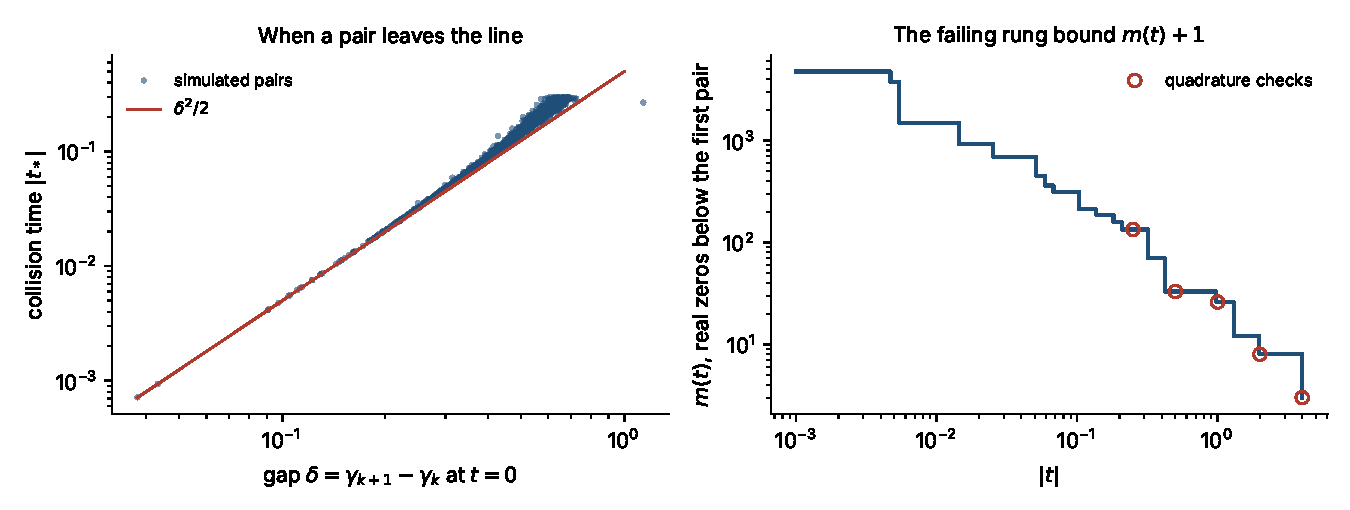
\includegraphics[width=\textwidth]{fig/v3/pf_fig_lehmer.pdf}
\caption{Left: the collision time of each pair against its gap at $t=0$, with the isolated pair law $\delta^2/2$. Right: $m(t)$ from the zero flow, with the quadrature checks.}
\label{p:fig:lehmer}
\end{figure}

\paragraph{Comparison with the Csordas Smith Varga bound} Csordas, Smith and Varga \cite{CSV94} turned the collision picture into a theorem.

\begin{theorem}[Csordas, Smith and Varga]\label{p:thm:csv}
Let $x_k<x_{k+1}$ be consecutive simple positive zeros of $H_0$, let $\Delta=x_{k+1}-x_k$ and
\[
g_k=\sum_{j\ne k,k+1}\Big[\frac1{(x_k-x_j)^2}+\frac1{(x_{k+1}-x_j)^2}\Big],
\]
the sum over all other zeros of both signs, with multiplicity. If $0<\Delta^2g_k<\frac45$ (a Lehmer pair), then
\[
\Lambda\ \ge\ \lambda_k=\frac{\big(1-\frac54\Delta^2g_k\big)^{4/5}-1}{8g_k}.
\]
\end{theorem}

To leading order $\lambda_k=-\frac18\Delta^2=-\frac12\delta^2$, the isolated pair law. We computed $g_k$ and $\lambda_k$ for the first $8900$ pairs, summing over the zeros we computed. There are $479$ Lehmer pairs, $5.4$ per cent of all pairs, and $477$ of them collide in the simulated range. The best bound from these zeros is $\lambda_{6709}\approx-7.11\times10^{-4}$, from Lehmer's original pair. A rigorous value needs a bound on the omitted tail, which Csordas, Smith and Varga supply in their paper; our truncated sum is not such a bound. The theorem is proved by contradiction from $\Lambda<\lambda_k$, which makes some collision happen no later than $\lambda_k$ but does not say that the collision of a particular pair is no later. So it does not bound each simulated $t_*$. The ratio $t_*/\lambda_k$ has median $0.98$ and minimum $0.89$, so the bound is close to the simulation for most pairs. For the closest pairs the simulated $|t_*|$ exceeds $|\lambda_k|$ by up to $0.35$ per cent (for the pair at $7005$, $7.137$ against $7.112$, in units of $10^{-4}$), for a cause not known.

Three facts emerge from Table~\ref{p:tab:lehmer} and Figure~\ref{p:fig:lehmer}.
\begin{itemize}
\item The isolated pair law is accurate for close pairs: the median of $|t_*|/(\delta^2/2)$ is $1.01$ over the $19$ pairs with $\delta<0.15$, and $1.17$ for $0.3<\delta<0.6$, where the outer neighbours hold the pair apart.
\item Heuristically $m(t)$ is the index of the lowest pair with $\delta\lesssim\sqrt{2|t|}$, so the failing rung near $t=0$ is set by record small gaps, and every new record close pair raises the ladder.
\item A least squares fit to the rows of Table~\ref{p:tab:lehmer} gives about $60\,|t|^{-0.64}$ (computed from the table rows; the window $10^{-3}\le|t|\le0.3$ is short). A random matrix count suggests growth near $|t|^{-3/2}$ up to logarithms, and the window cannot separate the two. The growth rate of $m(t)$ is open.
\end{itemize}
In the language of the ladder, Newman's conjecture ($\Lambda\ge0$, proved by Rodgers and Tao) says that some rung fails for every $t<0$, and RH says that at $t=0$ no rung fails however close the pairs. A mechanism that proves every rung at $t=0$ must therefore be insensitive to how small the gaps are; heuristically, it cannot work with a margin proportional to the gap.

\subsection{Is the rung bound sharp? The cases \texorpdfstring{$t=-4$}{t = -4} and \texorpdfstring{$t=-2$}{t = -2}}\label{p:sec:sharp}

Theorem~\ref{p:thm:heat} gives only the upper bound $r(t)\le m(t)+1$. We tested sharpness at $t=-4$, where $m=3$, and at $t=-2$, where $m=8$, by computing $F_t$ itself.

\paragraph{The density} For real $\tau$, $H_t(2i\tau)=\int_0^\infty e^{tu^2}\Phi(u)\cosh(2\tau u)\,\mathrm du$ has a positive integrand, so $\omega_t(\tau)=H_t(0)/H_t(2i\tau)$ is computed stably ($1600$ Gauss Legendre nodes on $[0,2]$, $256$ bits, $0\le\tau\le100$, where $\omega_{-4}(100)$ is below $10^{-50}$). Then $F_t$, $F_t'$ and $F_t''$ follow by the trapezoid rule, which is spectrally accurate because $\omega_t$ is even and analytic in a strip. For large $x$ we use the finite residue expansion over the zeros $z_k$ of $H_t$ below a cutoff, found by Newton's method in $200$ bit arithmetic,
\[
F_t(x)\approx\sum_k c_k e^{-z_kx/2},\qquad c_k=-\frac{H_t(0)}{2H_t'(z_k)},\qquad x>0,
\]
whose remainder is of the type \eqref{p:eq:residue}. The two agree to twelve digits at $x=2,3$ and to eight digits at $x=4$.

\paragraph{The zeros} The real zeros of $H_{-4}$ below the first pair are $30.622$, $45.200$, $52.289$, with residues $592$, $-7.7\times10^4$, $8.6\times10^5$, alternating in sign as for a P\'olya frequency function. The pair is $z=66.2302\pm0.3011\,i$, barely off the line, followed by real zeros at $78.709$, $86.525$, $87.045,\dots$. The pair sits inside the Laguerre interval $[52.3,78.7]$ of Table~\ref{p:tab:heat}.

\paragraph{The rungs} All of the following is computed.
\begin{itemize}
\item PF$_1$ and PF$_2$. $F_{-4}>0$ and $(\log F_{-4})''<0$ at every grid point of $[0,4]$ (step $0.01$), and the $2\times2$ minors in the far field are positive on the scanned shifts $L\in[0,90]$. Log concavity beyond $x=4$ is not proved: the leading one mode terms cancel in $FF''-F'^2$, so the two mode term must be compared with explicit bounds on the remainder.
\item PF$_3$. A random search over $2\times10^4$ configurations in the near field, followed by descent, found no negative $3\times3$ minor; all were rechecked in $50$ digit arithmetic. In the far field the $3\times3$ minors with $x_i=L+(0,\frac12,1)$ and $y_l=(0,\frac12,1)$ are positive at every scanned $L\in[3,90]$.
\item PF$_4$. The $4\times4$ minor with $x_i=L+(0,\frac12,1,\frac32)$ and $y_l=(0,\frac12,1,\frac32)$ changes sign at $L\approx23.5$, $44.0$, $65.0$ and $86.0$ (Figure~\ref{p:fig:rung}), located to the grid step $0.5$ and unchanged between $2500$ and $5000$ digit arithmetic.
\end{itemize}
So at $t=-4$ the evidence is that $r(-4)=4=m+1$ and the bound of Theorem~\ref{p:thm:heat} is attained. It is evidence only, because PF$_3$ was not tested on all of $\mathbb R^6$.

\paragraph{The case $t=-2$} The same computation finds eight real zeros of $H_{-2}$ at $29.44$, $43.59$, $51.18$, $62.92$, $66.66$, $76.89$, $83.68$, $87.39$ and then the pair $z=99.4309\pm0.4972\,i$. In the far field, with $x_i=L+\frac i2$ and $y_l=\frac l2$, the minor of order $9$ changes sign at $L\approx17.75$, $30.25$, $43.0$ and $55.5$ (grid step $0.25$, at $8000$ digits). The minor of order $8$ was checked at $L=6,24,42,60$ only, where it is positive. The near field was searched at orders $3$ and $4$ only, and the rungs $5$ to $8$ were not searched there. Here the evidence for sharpness is the far field alone.

\begin{corollary}[the detection scale]\label{p:cor:scale}
In the setting of Theorem~\ref{p:thm:detect}, let the lowest pair off the line have exponents $a\pm ib$ ($b=d$ for $\xi$). For a fixed configuration with $P\ne0$ the minor of order $m+1$ at shift $L$ equals $e^{-RL}\big(2|P|\cos(bL+\theta)+O(e^{-\eta L})\big)$ as $L\to\infty$, with $\theta=-\arg P$. Its large sign changes are asymptotically equally spaced at distance $\pi/b+o(1)$, and it is negative on intervals of that length.
\end{corollary}

\begin{proof}
This is the leading term in the proof of Theorem~\ref{p:thm:detect}. The same bound holds for the derivative in $L$, so the sign changes are simple and near the zeros of the cosine.
\end{proof}

Here $b=\frac12\Im z$, and the failing rung equals $m+1$ in both cases ($t=-4$, rung $4$; $t=-2$, rung $9$); the spacings between sign changes ($20.5$ to $21.0$, and $12.5$ to $12.75$) match $\pi/b=20.87$ and $12.64$ to within the grid step in $L$.

\begin{figure}[t]
\centering
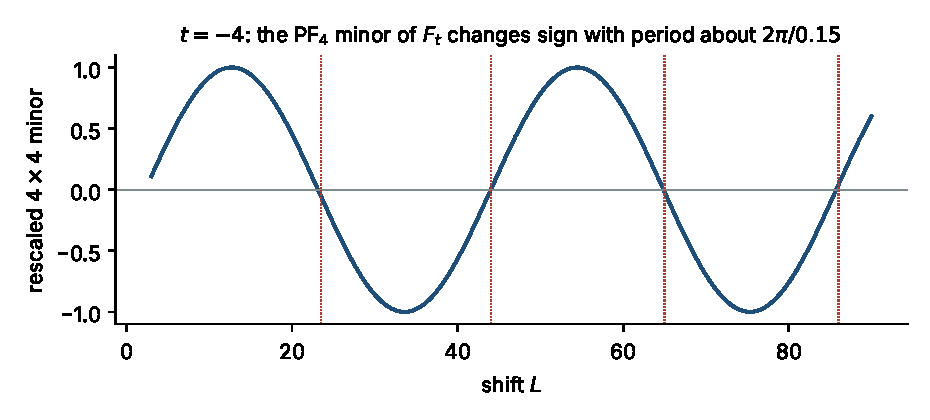
\includegraphics[width=\textwidth]{fig/v3/pf_fig_rung.pdf}
\caption{The $4\times4$ minor of $F_{-4}$ with $x_i=L+(0,\frac12,1,\frac32)$ and $y_l=(0,\frac12,1,\frac32)$, multiplied by $e^{(\lambda_1+\lambda_2+\lambda_3+\Re\lambda_4)L}$ with $\lambda_k=z_k/2$. It is a cosine of period $2\pi/\Im\lambda_4=41.7$.}
\label{p:fig:rung}
\end{figure}

\paragraph{Where the failure lives} The failure is invisible in the near field. At $t=-4$ it appears at shifts $L\approx23$, where the entries of the matrix are of size about $10^{-150}$ and the minor about $10^{-950}$ (computed). For a hypothetical zero $\beta+i\gamma$ of $\zeta$ off the critical line, $b=\beta-\frac12$, and the verification of RH to height $3\times10^{12}$ forces any such zero to lie at enormous height. In practice no finite computation on $F$ can find a counterexample this way, though a negative minor has finite order, coordinates and $L$, and could be certified in ball arithmetic. A proof of RH through the ladder has to be structural.

\section{Milestones and status}\label{p:sec:milestones}

\begin{enumerate}
\item PF$_1$ and PF$_2$ on $\mathbb R$: done, certified (Theorem~\ref{p:thm:m1}).
\item PF$_3$. Every $3\times3$ minor $\det[F(x_i-y_l)]$ with ordered points must be nonnegative. Translation invariance $(x_i,y_l)\mapsto(x_i+c,y_l+c)$ is one invariance, which leaves five parameters. In the far field, Theorem~\ref{p:thm:farpfk} with explicit constants, in the style of Section~\ref{p:sec:m1}, decides the minor from the residues of $\gamma_1,\gamma_2,\gamma_3$. In the near field, Taylor models of the minor can use the derivatives $F^{(j)}(a)$ computed on the grid. The new difficulty is the mixed configurations, in which some differences $x_i-y_l$ lie in each field.
\item Uniformity. By Corollary~\ref{p:cor:detect} the certificates of single rungs are not the content of the path. One would want a near field bound for PF$_k$ that follows from PF$_{k-1}$ together with real axis data, for instance through Karlin's composition formula for totally positive kernels \cite{Karlin68}.
\item Mechanism. A mechanism exists for the deformed densities $F_t$, $t\ge0.2$ (Theorem~\ref{p:thm:heat}). One would want a variation diminishing operator built from the primes and the gamma function with kernel $F$. Two candidates, products of Euler factors at a fake prime $P\downarrow1$ and the Curry Schoenberg B spline limit with knots from prime data, are worked through in Chapter~\ref{c:ch:cand}, and both fail in their naive form.
\end{enumerate}

A proof of RH along this path would need an argument that every PF$_k$ holds in the near field, uniformly in $k$, with the arithmetic of $\xi$ entering in an essential way, and, as research aims, an explanation of the tight spots, the first gap $(\gamma_1,\gamma_2)$ and the Lehmer type pairs, where the residues are inflated.

\section{Open problems}\label{p:sec:open}

\begin{enumerate}
\item Certify PF$_3$ on $\mathbb R^6$ (five parameters after translation), with explicit constants in Theorem~\ref{p:thm:farpfk} and a box decomposition of the mixed configurations. By Corollary~\ref{p:cor:detect} its value is structural rather than a new fact about zeros.
\item Does the control fail some rung $k\le43$ in the near field? The far field fails rung $44$ (Theorem~\ref{p:thm:detect}), and sampling for $k\le4$ found nothing.
\item An analytic proof of log concavity of $F$, in the sense of a proof by structure and not by certificate. The control is numerically log concave on the range computed, so such a proof should apply to a class of functions with a functional equation whose low zeros are on the line, and a precise hypothesis (not only alternating low residues) is part of the problem.
\item Make the Lehmer heuristic precise: bound the margin of rung $m+1$ in terms of the gap of the $(m+1)$th pair.
\item A uniform mechanism on $0\le t\le0.2$ with constants uniform as $t\downarrow0$.
\item The failing rung function. Certify the flow values rigorously (the tail bound and the lowest pair), extend beyond height $9000$, and determine the growth of $m(t)$ as $t\uparrow0$.
\item Is the rung bound sharp? Prove that $F_t$ passes every rung up to $m(t)$, which would make $r(t)=m(t)+1$ a theorem. It is a finite analogue of RH for each $t<0$.
\item Is $r(t)$ monotone in $t$? De Bruijn's theorem makes PF$_\infty$ propagate upward in $t$. Whether each finite rung does is open, and the order of the collisions in Table~\ref{p:tab:lehmer} shows that $m(t)$ need not be monotone in the model.
\end{enumerate}
